\documentclass[%
	corpo=11pt,
    twoside,
    stile=classica,
    oldstyle,
    tipotesi=custom,
    greek,
    evenboxes,
]{toptesi}
%%%%%%%%%%%%%%%%%%%%%%%%%%%%%%%%%%%%%%%%%%%%%%%%%%%%

\usepackage[utf8]{inputenc}
\usepackage[T1]{fontenc}
\usepackage{lmodern}

\usepackage{graphicx}
\usepackage{verbatim}
\usepackage{amsmath}
\usepackage{enumitem}

\usepackage{hyperref}
\hypersetup{%
    pdfpagemode={UseOutlines},
    bookmarksopen,
    pdfstartview={FitH},
    colorlinks,
    linkcolor={blue},
    citecolor={blue},
    urlcolor={blue}
  }

%%%%%%% use PDFLATEX 

\usepackage{lipsum} %to insert random text

\usepackage{geometry} %for the margins
\newcommand\fillin[1][4cm]{\makebox[#1]{\dotfill}} %for the dotted line in the frontispiace

\usepackage{dcolumn}
\newcolumntype{d}{D{.}{.}{-1} } %to vetical align numbers in tables, along the decimal dot

%\usepackage{amsmath}

\usepackage{natbib} % for the bibliography
\bibliographystyle{plainnat}


%%%%%%% Local definitions
\newtheorem{osservazione}{Osservazione}% Standard LaTeX
\newtheorem{observation}{Observation}% Standard LaTeX


%%%%%%% Custom fonts for title page
\newcommand\customfont[1]{{\usefont{T1}{Poppins-Regular}{m}{n} #1 }}

%%%%%%%%%%%%%%%%%%%%%%%%%%%%%%%%%%%%%%%%%%%%%%%%
%%%%%%%%%%%%%%%%%%%%%%%%%%%%%%%%%%%%%%%%%%%%%%%%



\begin{document}\errorcontextlines=9
%\english

\begin{titlepage}
\newgeometry{left=1cm,right=1cm,top=3cm,bottom=3.5cm}  %specific margins for this page

\begin{center}

{\huge POLITECNICO DI TORINO}\\[1.5cm]
\textbf{Corso di Laurea\\in Matematica per l'Ingegneria}\\[3cm]
%\textbf{Corso di Laurea Magistrale\\in Ingegneria Matematica}\\[3cm]

{\Large Tesi di Laurea}\\[1cm]
%{\Large Tesi di Laurea Magistrale}\\[0.5cm]
\textbf{\LARGE Titolo }\\[2cm]

\includegraphics[width=0.2\textwidth]{./Pictures/logo_polito_2021.jpg}
\vspace{4cm}

\customfont{hello world!}

\begin{minipage}{0.85\textwidth}
\begin{flushleft}\large
\textbf{Relatori} \hfill \textbf{Candidato}\\
prof. Nome Cognome \hfill Nome Cognome\\
prof. Nome Cognome \\
\textit{firma dei relatori} \hfill \textit{firma del candidato}\\[0.35cm]
\fillin\ \hfill \\
\fillin\ \hfill \fillin
\end{flushleft}
\end{minipage}

\vfill

Anno Accademico 2018-2019
\end{center}

\restoregeometry %restor default margins 

\end{titlepage} %the frontispiece

%%%%%%% Dedication
%\ifclassica%
%{\begin{dedica}
    %A mio padre

    %\textdagger\ A mio nonno Pino
%\end{dedica}
%%%%%%% 

\sommario%summary
%Here goes the abstrat of your thesis
Questa tesi esplora il ruolo delle copule nella modellazione della dipendenza tra variabili casuali, con particolare attenzione alle applicazioni in finanza. Dopo un'introduzione ai concetti fondamentali delle copule e alla loro teoria matematica, vengono analizzate diverse famiglie di copule, le loro proprietà e il loro utilizzo nella gestione del rischio finanziario. Successivamente, si discutono i metodi di stima dei parametri delle copule, con un focus su metodi classici e bayesiani, e si presenta un’implementazione pratica sui dati finanziari del DAX. Infine, vengono confrontati i risultati ottenuti con diverse copule e si discutono le implicazioni per la gestione del rischio e l’ottimizzazione di portafoglio.

%%%%%%%%%%%%%%%%%%%%%%%%%%%%%%%%%%%%%%%%%%%%%%%%
%%%%%%%%%%%%%%%%%%%%%%%%%%%%%%%%%%%%%%%%%%%%%%%%

\ringraziamenti%acknowledgements
%Acknowledge the people you love and/or work with
Da scrivere

%%%%%%%%%%%%%%%%%%%%%%%%%%%%%%%%%%%%%%%%%%%%%%%%
%%%%%%%%%%%%%%%%%%%%%%%%%%%%%%%%%%%%%%%%%%%%%%%%

%\tablespagetrue\figurespagetrue%to include the list of tables
%and the list of figures - yuo can comment these commands

\indici%table of content
%It automatically generated

%%%%%%%%%%%%%%%%%%%%%%%%%%%%%%%%%%%%%%%%%%%%%%%%
%%%%%%%%%%%%%%%%%%%%%%%%%%%%%%%%%%%%%%%%%%%%%%%%

%Citation
%If you feel like a poetic guy!
%\ifclassica   
%\begin{citazioni}
 %   \textit{If you cannot understand my\\argument, and declare}\\
  %  it's Greek to me\\
   % \textit{you are quoting Shakespeare.}
    
    %[\textsc{B. Levin}, Quoting Shakespeare]\vspace{1em}
%\end{citazioni}
%\fi

%%%%%%%%%%%%%%%%%%%%%%%%%%%%%%%%%%%%%%%%%%%%%%%%
%%%%%%%%%%%%%%%%%%%%%%%%%%%%%%%%%%%%%%%%%%%%%%%%

\mainmatter

\part{Fondamenti delle Copule}

\chapter{Introduzione}

\section{Definizione e motivazione dello studio}
Le copule sono strumenti matematici che permettono di modellare e stimare la dipendenza tra diverse variabili casuali. Sono particolarmente utili in finanza, dove la dipendenza tra i rendimenti degli asset, i tassi di interesse e i tempi di default sono fattori cruciali per la valutazione del rischio e la determinazione del prezzo di strumenti finanziari complessi. L’importanza delle copule risiede nella loro capacità di separare la modellazione delle distribuzioni marginali delle singole variabili dalla modellazione della loro struttura di dipendenza.

In altre parole, invece di dover specificare una funzione di distribuzione congiunta per tutte le variabili, è possibile utilizzare una copula per combinare le distribuzioni marginali di ciascuna variabile in una distribuzione congiunta che rifletta la dipendenza desiderata. Questo approccio offre grande flessibilità nella modellazione, poiché consente di scegliere le distribuzioni marginali e la copula in modo indipendente, a seconda delle caratteristiche specifiche dei dati e del problema in esame.

Ad esempio, si potrebbe utilizzare una distribuzione t di Student per modellare i rendimenti degli indici azionari, che spesso presentano code più spesse rispetto alla distribuzione normale, e quindi utilizzare una copula di Gumbel per rappresentare la dipendenza asimmetrica tra i mercati, con una maggiore probabilità di movimenti congiunti al rialzo rispetto a quelli al ribasso.

La teoria delle copule si basa sul teorema di Sklar, che afferma che ogni funzione di distribuzione congiunta può essere espressa in termini di una copula e delle distribuzioni marginali delle variabili. Il teorema di Sklar garantisce l’esistenza e l’unicità della copula nel caso di variabili casuali continue. 

Esistono diverse famiglie di copule, ciascuna con proprietà specifiche in termini di dipendenza di coda, simmetria e altre caratteristiche. Alcune delle famiglie di copule più utilizzate in finanza includono la copula gaussiana, la copula t di Student, le copule Archimedee (come la copula di Gumbel, la copula di Clayton e la copula di Frank) e la copula di Marshall-Olkin. La scelta della copula più adatta dipende dalla natura del problema e dalle caratteristiche della dipendenza che si desidera modellare.

Ad esempio, la
copula t di Student é spesso preferita alla copula gaussiana quando si vogliono
modellare dipendenze di coda più
elevate, mentre le copule Archimedee consentono di modellare diversi tipi di dipendenza asimmetrica.

Le copule trovano applicazione in diversi ambiti della finanza, tra cui:

\begin{itemize}
	\item \textbf{Pricing di opzioni multivariate e altri derivati}: le copule possono essere utilizzate per modellare la dipendenza tra i sottostanti di un’opzione basket, un’opzione rainbow o altri derivati multi-asset, consentendo una valutazione più accurata del prezzo di questi strumenti.
	
	\item \textbf{Gestione del rischio}: le copule sono ampiamente utilizzate nella modellazione del rischio di credito, dove consentono di stimare la probabilità di default congiunta di diverse attività o controparti. Le copule sono anche utilizzate nella stima del Value at Risk (VaR) di portafogli contenenti attività con distribuzioni non normali e dipendenze complesse.
	
	\item \textbf{Calibrazione e simulazione}: la flessibilità delle copule consente di calibrare i modelli ai dati di mercato in modo efficiente e di simulare scenari di mercato realistici che tengano conto della dipendenza tra le variabili.
\end{itemize}

In sintesi, le copule rappresentano uno strumento matematico versatile e potente per la modellazione della dipendenza in finanza, con un ampio spettro di applicazioni pratiche nella valutazione del rischio, nel pricing di derivati e nella gestione del portafogli.


\chapter{Fondamenti Matematici delle Copule}

\section{Definizione di copula e Teorema di Sklar}

Le copule sono strumenti matematici che permettono di modellare e rappresentare la dipendenza tra variabili casuali. A differenza di misure di dipendenza tradizionali come la correlazione lineare, le copule catturano la dipendenza in modo più completo, includendo la dipendenza nelle code delle distribuzioni e non limitandosi a relazioni lineari.

Ecco una spiegazione delle formule e delle proprietà chiave:

\subsection{Definizione di Copula}
Una \(d\)-copula è una funzione \( C : [0,1]^d \to [0,1] \), dove \( d \geq 2 \) (numero di variabili; nelle proprietà seguenti consideriamo le copule bivariate), che soddisfa le seguenti proprietà:

\begin{enumerate}
	\item \textbf{Groundedness:}  
	\[
	C(u,0) = C(0,v) = 0, \quad \forall u, v \in [0,1]^2
	\]
	Ciò significa che la copula è zero se una delle variabili è zero.
	
	\item \textbf{Marginalità:}  
	\[
	C(u,1) = u, \quad C(1,v) = v, \quad \forall u, v \in [0,1]^2
	\]
	Questa proprietà assicura che la copula sia coerente con le distribuzioni marginali, ovvero che quando una delle variabili assume il suo valore massimo, la copula coincida con la funzione di ripartizione dell’altra variabile.
	
	\item \textbf{2-crescita (o 2-increasing):}  
	\[
	C(u_2,v_2) - C(u_2,v_1) - C(u_1,v_2) + C(u_1,v_1) \geq 0, \quad \forall u_1 \leq u_2, v_1 \leq v_2 \in [0,1]^2
	\]
	Questa proprietà assicura che la copula sia non decrescente in entrambe le variabili, il che è necessario affinché la copula rappresenti una dipendenza positiva o negativa tra le variabili.
\end{enumerate}

\subsection{Teorema di Sklar}
Questo teorema, centrale nella teoria delle copule, stabilisce un legame tra le copule e le funzioni di distribuzione congiunta.  

In breve, il teorema afferma che:  
Data una funzione di distribuzione congiunta \( F(x,y) \) con marginali \( F_1(x) \) e \( F_2(y) \), esiste una copula \( C \) tale che:
\[
F(x,y) = C(F_1(x), F_2(y))
\]
Inoltre, se \( F_1(x) \) e \( F_2(y) \) sono continue, allora la copula \( C \) è unica.

\subsubsection{Conseguenze del Teorema di Sklar}
\begin{itemize}
	\item \textbf{Costruzione di modelli di dipendenza:}  
	Permette di costruire una funzione di distribuzione congiunta a partire da distribuzioni marginali arbitrarie e da una copula che ne modella la dipendenza. Questa proprietà è particolarmente utile per modellare dati reali, dove spesso si conoscono le distribuzioni marginali ma non la struttura di dipendenza.
	
	\item \textbf{Separazione tra marginali e dipendenza:}  
	Mette in luce come la struttura di dipendenza tra le variabili sia completamente catturata dalla copula, indipendentemente dalle distribuzioni marginali.
\end{itemize}


\section{Famiglie principali di copule (Gaussiane, t-Student, Archimedee) }

\subsection{Famiglie di copule}
Esistono diverse famiglie di copule, classificate in base alla loro struttura o ai metodi utilizzati per la loro costruzione. Di seguito, vengono elencate alcune delle principali famiglie:

\begin{itemize}
	\item \textbf{Fréchet-Hoeffding:} Questa famiglia include le copule che rappresentano i limiti inferiore (\(W\)) e superiore (\(M\)) della dipendenza tra due variabili casuali. La copula \(W\) rappresenta la perfetta dipendenza negativa, mentre la copula \(M\) rappresenta la perfetta dipendenza positiva.
	
	\item \textbf{Cuadras-Augé:} Questa famiglia di copule è costruita come una media geometrica ponderata delle copule \(M\) e \(P\), dove \(P\) rappresenta l’indipendenza tra le variabili.
	
	\item \textbf{Marshall-Olkin:} Questa famiglia di copule è spesso utilizzata per modellare la dipendenza tra variabili casuali che rappresentano tempi di vita.
	
	\item \textbf{Archimedee:} Queste copule sono generate da una funzione detta "generatore". Le copule Archimedee sono popolari per la loro flessibilità e la relativa facilità di utilizzo.
\end{itemize}

\subsection{Proprietà delle copule}
Le copule possiedono diverse proprietà che le rendono utili per la modellazione della dipendenza. Alcune di queste proprietà sono:

\begin{itemize}
	\item \textbf{Invarianza rispetto a trasformazioni monotone crescenti:}  
	Le copule sono invarianti rispetto a trasformazioni strettamente crescenti delle variabili marginali.
	
	\item \textbf{Misure di concordanza:}  
	Diverse misure di concordanza come la rho di Spearman e la tau di Kendall possono essere espresse in termini di copule.
	
	\item \textbf{Dipendenza di coda:}  
	Le copule possono catturare la dipendenza tra le code delle distribuzioni marginali, ovvero la tendenza delle variabili ad assumere valori estremi congiuntamente.
\end{itemize}

Possiamo quindi affermare che le copule offrono un approccio potente e flessibile per la modellazione della dipendenza tra variabili casuali. La loro capacità di separare la struttura di dipendenza dalle distribuzioni marginali, la loro invarianza rispetto a trasformazioni monotone crescenti e la loro capacità di catturare la dipendenza di coda le rendono strumenti preziosi in molte applicazioni pratiche.




\part{Applicazioni Finanziarie delle Copule}

\chapter{Copule e Gestione del Rischio Finanziario}

\section{Superamento della correlazione lineare nelle distribuzioni non normali}

L'assunzione di normalità dei rendimenti, tipico di modelli come quello di Black-Scholes, è spesso disatteso nei mercati finanziari. Le serie storiche di strumenti come azioni ed obbligazioni dimostrano la presenza di code più pesanti rispetto a quanto previsto dalla distribuzione normale e la diffusione di prodotti derivati con payoff non lineari amplifica ulteriormente questo fenomeno.

In questo contesto, la \textbf{correlazione lineare}, misurata ad esempio con il coefficiente di Pearson, si dimostra uno strumento limitato. Essa cattura solo le dipendenze lineari tra le variabili, mentre le relazioni tra gli asset finanziari possono assumere forme ben più complesse. La correlazione lineare è efficace solo quando le variabili sono legate da relazioni lineari. Tuttavia, in presenza di legami non lineari, la correlazione lineare potrebbe essere fuorviante. Ad esempio, una variabile con distribuzione chi-quadrato è perfettamente correlata al suo quadrato, che ha distribuzione normale, ma la correlazione lineare non sarebbe in grado di rappresentare correttamente questa relazione.

\subsection{Coefficiente di Pearson}

Il coefficiente di correlazione lineare, noto anche come correlazione di Pearson, è una misura della dipendenza lineare tra due variabili casuali che assumono valori reali e che hanno varianza finita. È definito come la covarianza delle due variabili divisa per il prodotto delle loro deviazioni standard. Formalmente, per due variabili casuali non degeneri \( X \) e \( Y \) appartenenti a \( L^2 \), il coefficiente di correlazione lineare \( \rho_{XY} \) è:

\[
\rho_{XY} = \frac{\text{cov}(X,Y)}{\sqrt{\text{var}(X)\text{var}(Y)}}
\]
\newline
Il coefficiente di correlazione di Pearson assume valori compresi tra -1 e +1, dove:
\begin{itemize}
	\item \( +1 \) indica una perfetta correlazione lineare positiva: all’aumentare di una variabile, l’altra aumenta in modo perfettamente lineare.
	\item \( -1 \) indica una perfetta correlazione lineare negativa: all’aumentare di una variabile, l’altra diminuisce in modo perfettamente lineare.
	\item \( 0 \) indica l’assenza di correlazione lineare: non c’è una relazione lineare tra le due variabili.
\end{itemize}

È importante sottolineare che il coefficiente di correlazione di Pearson misura solo la dipendenza lineare. Due variabili possono essere fortemente dipendenti in modo non lineare e avere comunque un coefficiente di correlazione di Pearson pari a zero.

\subsection{Vantaggi delle Copule rispetto alla Correlazione Lineare}
Le \textbf{copule}, invece, offrono un approccio più flessibile per modellare la dipendenza tra variabili casuali, anche in presenza di distribuzioni non normali. Il vantaggio principale delle copule risiede nella loro capacità di separare la struttura di dipendenza dalle distribuzioni marginali. Questo permette di combinare diverse distribuzioni marginali, capaci di cogliere la non-normalità dei rendimenti (ad esempio la distribuzione t di Student o distribuzioni asimmetriche), con una vasta gamma di copule che descrivono la struttura di dipendenza.

Il \textbf{Teorema di Sklar}, fondamento della teoria delle copule, afferma che ogni funzione di distribuzione congiunta può essere espressa in termini di distribuzioni marginali e di una copula. Questa proprietà permette di costruire modelli di dipendenza altamente flessibili, adatti a rappresentare le complesse relazioni tra gli asset finanziari. Ad esempio, è possibile utilizzare una copula gaussiana per modellare la struttura di dipendenza, pur mantenendo distribuzioni marginali non gaussiane per i singoli asset. In questo modo, si ottiene un modello in grado di catturare sia la non-normalità dei rendimenti sia le strutture di dipendenza tra gli stessi.

In definitiva, le copule rappresentano uno strumento più completo e affidabile rispetto alla correlazione lineare per modellare le dipendenze tra variabili casuali, soprattutto in presenza di distribuzioni non normali. La loro flessibilità e capacità di rappresentare accuratamente le complesse relazioni tra gli asset le rendono essenziali per una corretta valutazione del rischio, un pricing accurato e una migliore comprensione delle dinamiche dei mercati finanziari.
\newpage
\section{Dipendenza di coda e impatti su Value-at-Risk (VaR) e Expected Shortfall}

La dipendenza di coda si riferisce alla tendenza di due o più variabili casuali a muoversi insieme in modo più estremo nelle code delle loro distribuzioni, rispetto a quanto previsto da una distribuzione normale con la stessa correlazione lineare. In altre parole, la dipendenza di coda misura la probabilità che si verifichino eventi estremi congiuntamente.

Sappiamo che la non normalità a livello univariato è associata al cosiddetto problema della \textit{fat-tail}. In un contesto multivariato, il problema della \textit{fat-tail} può essere riferito sia alle distribuzioni marginali univariate che alle distribuzioni congiunte di probabilità di grandi movimenti di mercato. Questo concetto è chiamato \textbf{tail dependence}. L’uso di funzioni copula ci permette di modellare separatamente queste due caratteristiche. Per rappresentare la dipendenza dalla coda consideriamo la probabilità che un evento con probabilità inferiore a \( v \) si verifichi nella prima variabile, dato che un evento con probabilità inferiore a \( v \) si verifica nella seconda. In concreto, ci chiediamo quale sia la probabilità di osservare, ad esempio, un crollo con probabilità inferiore di \( v=1\% \) nell’indice Nikkei 225, dato che nell’indice S\&P 500 si è verificato un crollo con probabilità inferiore all’1\%. Si ha:

\[
\lambda(v) \equiv \Pr(Q_{NKY} \leq v \mid Q_{SP} \leq v)
\]

\[
= \frac{\Pr(Q_{NKY} \leq v, Q_{SP} \leq v)}{\Pr(Q_{SP} \leq v)}
\]

\[
= \frac{C(v,v)}{v}
\]

\subsection{Tipi di dipendenza di coda}
Dopo che abbiamo calcolato il nostro \( \lambda(v) \), possiamo dividere la dipendenza di coda in due tipi principali:

\begin{itemize}
	\item \textbf{Dipendenza di coda inferiore}: misura la probabilità che entrambe le variabili assumano valori estremamente bassi contemporaneamente.
	\[
	\lambda_L \equiv \lim_{v \to 0^+} \frac{C(v,v)}{v}
	\]
	
	\item \textbf{Dipendenza di coda superiore}: misura la probabilità che entrambe le variabili assumano valori estremamente alti contemporaneamente.
	\[
	\lambda_U = \lim_{v \to 1^-} \lambda_v \equiv \lim_{v \to 1^-} \frac{\Pr(Q_{NKY} > v, Q_{SP} > v)}{\Pr(Q_{SP} > v)}
	\]
	
	\[
	= \lim_{v \to 1^-} \frac{1 - 2v + C(v,v)}{1 - v}
	\]
\end{itemize}

\subsection{Importanza nel VaR e nell’Expected Shortfall}
La dipendenza di coda ha un impatto significativo sul calcolo del \textbf{VaR} e dell’\textbf{Expected Shortfall}, due misure di rischio ampiamente utilizzate nella gestione del rischio finanziario.

\begin{itemize}
	\item \textbf{VaR (Value at Risk)}: rappresenta la perdita massima stimata che un portafoglio potrebbe subire in un determinato orizzonte temporale e con un dato livello di confidenza.
	\item \textbf{Expected Shortfall}: rappresenta la perdita media attesa in caso di superamento del VaR.
\end{itemize}

In presenza di dipendenza di coda, il VaR e l’Expected Shortfall calcolati assumendo una distribuzione normale tendono a sottostimare il rischio effettivo del portafoglio. Questo perché la distribuzione normale non riesce a catturare adeguatamente la probabilità di eventi estremi congiunti. Mentre utilizzando le copule per modellare la dipendenza tra gli asset di un portafoglio, è possibile ottenere una stima più accurata del VaR e dell’Expected Shortfall, tenendo conto della probabilità di eventi estremi congiunti. Quindi grazie alle copule è possibile una misura più accurata del rischio di portafoglio e si possono prendere decisioni più consapevoli.
\newpage
\section{Pricing di derivati multivariati con copule e gestione del rischio}

\subsection{Tariffare le opzioni}
La valutazione di opzioni multivariate, come le opzioni basket o rainbow, che dipendono da più attività sottostanti, rappresenta una sfida significativa in finanza. Le copule forniscono un potente strumento per affrontare questo problema.

\begin{itemize}
	\item In sostanza, una copula viene utilizzata per costruire la distribuzione congiunta dei prezzi delle attività sottostanti alla scadenza.
	\item Questa distribuzione viene quindi utilizzata per calcolare il valore atteso del payoff dell’opzione in base a tutti i possibili risultati dei prezzi delle attività sottostanti.
	\item Attualizzando questo valore atteso al tasso privo di rischio, si ottiene il prezzo dell’opzione.
\end{itemize}

Nei mercati incompleti, dove non esiste una misura di probabilità unica priva di arbitraggio, le copule sono fondamentali per derivare strategie di super-replicazione. Queste strategie mirano a creare un portafoglio di attività negoziabili che replichi il payoff dell’opzione in tutte le possibili situazioni future, garantendo così l’assenza di opportunità di arbitraggio. Le copule consentono di determinare i limiti superiori e inferiori del prezzo dell’opzione in base alle diverse ipotesi sulla struttura di dipendenza tra le attività sottostanti. Mostriamo ora degli esempi:

\begin{itemize}
	\item \textbf{Opzioni arcobaleno}: queste opzioni, che dipendono dal minimo o dal massimo di un paniere di attività, possono essere valutate utilizzando le copule per catturare la dipendenza tra i rendimenti delle attività. Le fonti dimostrano come le copule possano essere utilizzate per derivare strategie di super-replicazione per le opzioni arcobaleno, fornendo limiti superiori e inferiori al prezzo.
	
	\item \textbf{Opzioni barriera}: per le opzioni in cui l’esercizio è condizionato al fatto che il prezzo dell’attività sottostante raggiunga o meno una determinata barriera, le copule possono essere utilizzate per modellare la dipendenza tra il processo del prezzo dell’attività e l’evento di attivazione della barriera.
\end{itemize}

\subsection{Gestione dei rischi}
Le copule possono essere utilizzate per modellare la dipendenza tra diversi tipi di rischio, come rischio di mercato, rischio di credito e rischio operativo. Ciò è particolarmente utile per le istituzioni finanziarie che sono esposte a più tipi di rischio, in quanto consente loro di valutare il rischio complessivo a cui sono esposte. Ad esempio, una banca può utilizzare le copule per modellare la dipendenza tra le insolvenze sui prestiti e i movimenti dei tassi di interesse, consentendo loro di valutare il rischio del proprio portafoglio prestiti in diversi scenari economici.

In particolare, nella gestione del rischio di credito, le copule vengono utilizzate nella valutazione di strumenti di debito strutturati come le obbligazioni garantite da crediti (CDO). Le CDO sono obbligazioni garantite da un pool di attività sottostanti, come mutui o prestiti alle imprese. Il rischio di credito di una CDO dipende dalla dipendenza tra le insolvenze delle attività sottostanti. Le copule forniscono un modo flessibile per modellare questa dipendenza, consentendo agli investitori di valutare il rischio e il rendimento delle CDO in modo più accurato.

\section{Modelli di copula}

\subsection{Tipi di modelli di copula}
\begin{itemize}
	\item \textbf{Copula gaussiana}: descrive la dipendenza tra variabili casuali utilizzando la distribuzione normale multivariata. Non è in grado di catturare la dipendenza dalla coda. È definita come la funzione di distribuzione congiunta di un vettore normale multivariato standard, dove ogni variabile marginale è stata trasformata nella sua forma univariate standard utilizzando la funzione di distribuzione normale standard inversa.
	
	\[
	C_R^{Ga}(u,v) = \Phi_R(\Phi^{-1}(u), \Phi^{-1}(v))
	\]
	
	\[
	= \int_{-\infty}^{\Phi^{-1}(u)} \int_{-\infty}^{\Phi^{-1}(v)} \frac{1}{2\pi \sqrt{1-\rho_{XY}^2}} \exp \left( \frac{2\rho_{XY}st - s^2 - t^2}{2(1-\rho_{XY}^2)} \right) ds \, dt
	\]
	
	\item \textbf{Copula t di Student}: Questa copula può catturare la dipendenza dalla coda e viene spesso utilizzata per modellare i rendimenti degli asset che mostrano code pesanti. La copula t di Student bivariata è data dalla seguente formula:
	
	\[
	C_t(u,v) = \int_{-\infty}^{t_{\nu}^{-1}(u)} \int_{-\infty}^{t_{\nu}^{-1}(v)} \frac{\Gamma \left( \frac{\nu+2}{2} \right)}{\Gamma \left( \frac{\nu}{2} \right) \pi \nu \sqrt{1-\rho^2}} \left(1 + \frac{x^2 -2\rho xy + y^2}{\nu(1-\rho^2)}\right)^{-\frac{\nu+2}{2}} dx \, dy
	\]
	
	dove \( t_{\nu}^{-1} \) è l’inversa della funzione di distribuzione t di Student univariata con \( \nu \) gradi di libertà e \( \rho \) è il coefficiente di correlazione.
	
	\item \textbf{Copula di Clayton}: questa copula mostra una forte dipendenza dalla coda inferiore, il che significa che le variabili hanno maggiori probabilità di assumere insieme valori estremi bassi. È esaustiva e fornisce la copula del prodotto se \( \alpha = 0 \), il limite inferiore di Fréchet \( \max(v+z-1, 0) \) quando \( \alpha = -1 \) e quello superiore per \( \alpha \to +\infty \). È definita dalla seguente formula:
	
	\[
	C(v,z) = \max[(v^{-\alpha} + z^{-\alpha} - 1)^{-\frac{1}{\alpha}}, 0]
	\]
	
	\item \textbf{Copula di Gumbel}: questa copula mostra una forte dipendenza dalla coda superiore, indicando che le variabili hanno maggiori probabilità di assumere insieme valori estremi elevati. Fornisce la copula del prodotto se \( \alpha = 1 \) e il limite superiore di Fréchet \( \min(v,z) \) per \( \alpha \to +\infty \). È definita dalla seguente formula:
	
	\[
	C(v,z) = \exp \left( -[(-\ln v)^\alpha + (-\ln z)^\alpha]^{\frac{1}{\alpha}} \right)
	\]
	
	\item \textbf{Copula di Frank}: questa copula è una copula simmetrica che può catturare sia la dipendenza dalla coda superiore che quella dalla coda inferiore. Si riduce alla copula del prodotto se \( \alpha = 0 \) e raggiunge i limiti inferiori e superiori di Fréchet rispettivamente per \( \alpha \to -\infty \) e \( \alpha \to +\infty \). È definita dalla seguente formula:
	
	\[
	C(v,z) = -\frac{1}{\alpha} \ln \left( 1 + \frac{(e^{-\alpha v} - 1)(e^{-\alpha z} - 1)}{e^{-\alpha} - 1} \right)
	\]
	
\end{itemize}




\part{Preparazione dei Dati e Assunzioni}

\chapter{Preparazione dei Dati per la Modellazione con Copule}

\section{Struttura e caratteristiche dei dati}

Il seguente dataset contiene dati storici sul DAX, che rappresentano prezzi o indici di mercato rilevanti. La raccolta dati fornisce i valori di Open, High, Low, Close partendo dal giorno 02/01/2020 ore 01:15:00 e terminando con il giorno 03/03/2022 ore 09:14:00. La raccolta e la gestione adeguata di tali dati sono fondamentali per analizzare le dipendenze tra strumenti finanziari tramite modelli di copula. Tramite questi dati calcoleremo i rendimenti giornalieri, un passaggio necessario per la modellazione delle dipendenze.

\begin{figure}[h]
	\centering
	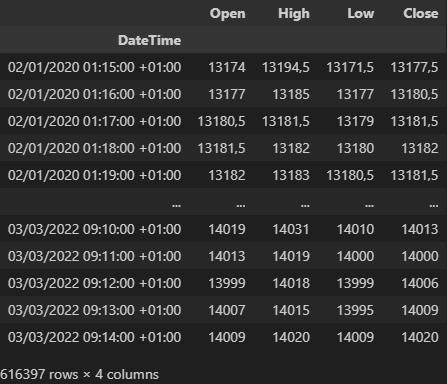
\includegraphics[width=0.6\textwidth]{./Pictures/dfDax.png}
	\caption{Inizio e fine del dataset}
	\label{fig:dataset}
\end{figure}

\section{Pulizia e preprocessing}

I dati finanziari spesso includono anomalie come valori mancanti o outlier che devono essere gestiti prima dell’analisi. Saranno implementate le seguenti tecniche di pulizia dei dati:
\begin{itemize}
	\item \textbf{Gestione dei valori mancanti}: rimuovere eventuali righe con valori mancanti per evitare distorsioni.
	\item \textbf{Gestione degli outlier}: utilizzare tecniche di filtraggio per identificare ed eliminare gli outlier, assicurando che l’analisi si concentri sui valori centrali più rappresentativi.
\end{itemize}
\textbf{Outlier}: nel contesto dei dati azionari, un outlier (o valore anomalo) è un’osservazione che si discosta significativamente dalla norma o dalla tendenza generale del dataset. In altre parole, si tratta di un dato che è molto diverso rispetto agli altri valori presenti nel campione.

Il motivo per cui vanno eliminati è che possono distorcere le analisi statistiche, poiché influenzano la media, la deviazione standard e altre misure di dispersione dei dati.

Ecco alcune righe di codice utilizzate per ``pulire'' i dati:
\begin{verbatim}
	import pandas as pd
	
	# Load the data
	data = pd.read_csv('DAX_3Y-1M.csv',index_col='DateTime',
	parse_dates=True)
	
	# Drop rows with missing values
	data=data.dropna()
	
	# Verifica e gestione degli outlier tramite interquartile
	range (IQR)
	Q1 = data.quantile(0.25)
	Q3 = data.quantile(0.75)
	IQR = Q3 - Q1
	filtered_data = data[~((data < (Q1 - 1.5 * IQR)) | 
	(data > (Q3 + 1.5 * IQR))).any(axis=1)]
\end{verbatim}

Circa 6000 righe di dati sono state eliminate da questo processo.
\newpage
\section{Trasformazione dei dati}

Dopo la pulizia, è necessario trasformare i dati per ottenere una scala uniforme. Poiché i modelli di copula richiedono margini uniformi, trasformeremo i dati in rendimenti logaritmici per ottenere stazionarietà e calcoleremo i punteggi standardizzati:

Ecco alcune righe di codice utilizzate per ``trasformare'' i dati:

\begin{verbatim}
	import numpy as np
	
	# Calcolo dei rendimenti logaritmici
	log_returns = np.log(filtered_data / filtered_data.shift(1)).dropna()
	
	# Standardizzazione dei dati
	# (sottraggo la media e divido per la deviazione standard)
	standardized_data = (log_returns - log_returns.mean()) / log_returns.std()
\end{verbatim}

\begin{figure}[h]
	\centering
	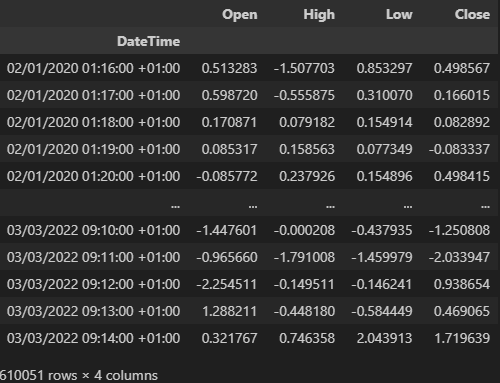
\includegraphics[width=0.8\textwidth]{./Pictures/dfnormal.png}
	\caption{Rendimenti logaritmici standardizzati}
	\label{fig:log_returns}
\end{figure}
\newpage
\section{Normalizzazione}

Per applicare correttamente i modelli di copula, i dati devono essere trasformati in una distribuzione uniforme sull’intervallo \([0,1]\). Questo passaggio permette ai dati di adattarsi meglio alla funzione di copula che verrà utilizzata per modellare le dipendenze:

\begin{verbatim}
	from scipy.stats import norm
	
	# Normalizzazione tramite la funzione di distribuzione cumulativa (CDF)
	uniform_data = norm.cdf(standardized_data)
\end{verbatim}

\begin{figure}[h]
	\centering
	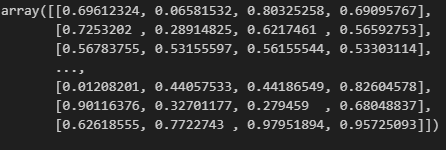
\includegraphics[width=0.8\textwidth]{./Pictures/norm.png}
	\caption{Dati uniformati all’intervallo [0,1]}
	\label{fig:uniform_data}
\end{figure}

\section{Assunzioni nei modelli di copula}

Per l’uso corretto dei modelli di copula, è essenziale discutere alcune assunzioni chiave:

\begin{itemize}
	\item \textbf{Uniformità marginale}: l’assunzione primaria nella modellazione delle copule è che le variabili marginali abbiano distribuzioni uniformi. Abbiamo utilizzato la funzione di distribuzione cumulativa per garantire questa uniformità.
	
	\item \textbf{Struttura di dipendenza}: i modelli di copula modellano la struttura di dipendenza tra le variabili senza fare ipotesi sui margini. Ciò significa che, dopo la trasformazione, possiamo utilizzare diversi tipi di copule per analizzare come i vari strumenti finanziari si muovono insieme.
	
	\item \textbf{Stazionarietà}: è importante che i dati siano stazionari, ovvero che le loro proprietà statistiche (come media e varianza) siano costanti nel tempo. Abbiamo utilizzato la differenziazione logaritmica per rendere i dati stazionari.
	
	\item \textbf{Normalità}: per l’utilizzo di una copula Gaussiana, i margini devono approssimare la normalità. Sebbene non sia strettamente necessario per altre copule come la t-Copula, una trasformazione per avvicinarsi alla normalità può essere utile per semplificare l’analisi.
\end{itemize}

\newpage

\section{Distribuzione dei rendimenti}

\begin{figure}[h]
	\centering
	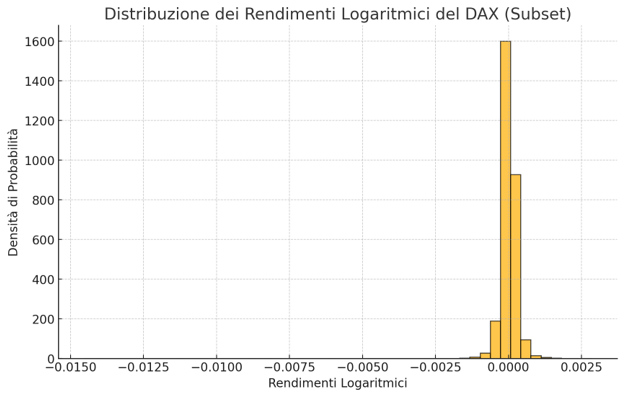
\includegraphics[width=0.8\textwidth]{./Pictures/rendimenti.png}
	\caption{Distribuzione dei Rendimenti Logaritmici del DAX (Subset)}
	\label{fig:log_returns_distribution}
\end{figure}

Ecco la distribuzione dei rendimenti logaritmici del DAX, calcolata su un subset dei dati disponibili. La distribuzione mostra la tipica forma a campana, con alcune code più pesanti, suggerendo la presenza di eventi estremi più frequenti rispetto a una normale distribuzione Gaussiana. Questa caratteristica supporta l’idea di utilizzare copule come la Student-t, che meglio cattura queste dipendenze nelle code.


Di seguito la matrice di correlazione tra i rendimenti logaritmici delle diverse colonne di prezzo (Open, High, Low, Close) sempre del subset.

\begin{figure}[h]
	\centering
	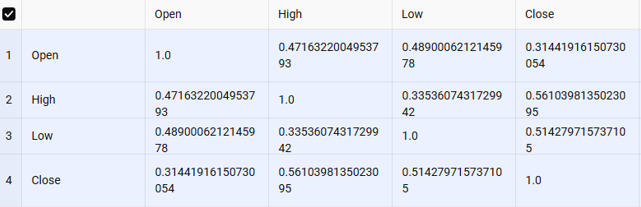
\includegraphics[width=0.8\textwidth]{./Pictures/corr.png}
	\caption{Matrice di correlazione}
	\label{fig:correlation_matrix}
\end{figure}

\section{Assunzioni generali}

Considerando i dati analizzati e i risultati ottenuti dalle elaborazioni, possiamo formulare le seguenti assunzioni per l’applicazione dei modelli di copula:

\begin{enumerate}
	\item \textbf{Uniformità marginale} \\
	Una delle assunzioni principali per applicare i modelli di copula è che le variabili marginali siano uniformi. Nel nostro caso, i rendimenti logaritmici calcolati per le diverse variabili (Open, High, Low, Close) sono stati trasformati in modo tale da poter essere considerati approssimativamente stazionari, ma non sono ancora stati resi uniformi. Per l’applicazione delle copule, sarà necessario trasformare i rendimenti normalizzati in una distribuzione uniforme sull’intervallo \([0,1]\), ad esempio usando la funzione di distribuzione cumulativa empirica. Questo passaggio garantisce che le dipendenze tra variabili siano modellate correttamente senza distorsioni derivanti dalle distribuzioni marginali.
	
	\item \textbf{Stazionarietà dei dati} \\
	Per applicare correttamente i modelli di copula, è necessario che le serie temporali siano stazionarie, ovvero che le proprietà statistiche come media e varianza siano costanti nel tempo. Abbiamo trasformato i prezzi in rendimenti logaritmici per ottenere una serie più stazionaria rispetto ai dati originali di prezzo. Tuttavia, è possibile che ci siano ancora componenti non stazionarie, come trend residui o stagionalità, che potrebbero influire sui risultati. La verifica e il trattamento di eventuali residui non stazionari sono fondamentali per garantire la validità dei modelli di copula.
	
	\item \textbf{Struttura di dipendenza} \\
	L’analisi dei rendimenti logaritmici ha mostrato una correlazione positiva tra le variabili, sebbene con valori differenti per ciascuna coppia (ad esempio, correlazione relativamente più alta tra High e Close, e più bassa tra Open e Close). Questa osservazione implica che esiste una struttura di dipendenza tra le variabili di prezzo, che va oltre la correlazione lineare. Le copule ci permetteranno di catturare meglio questa dipendenza, soprattutto nei casi in cui le correlazioni sono condizionate da situazioni estreme (code pesanti).
	
	\item \textbf{Dipendenze di coda} \\
	Osservando la distribuzione dei rendimenti logaritmici, è evidente che la distribuzione presenta code più pesanti rispetto a una normale distribuzione Gaussiana. Questo suggerisce una maggiore probabilità di eventi estremi (sia positivi che negativi), specialmente durante periodi di volatilità del mercato. Pertanto, è ragionevole assumere che le variabili presentino dipendenza di coda, rendendo modelli come la copula di Student-t o la copula di Clayton adatti per catturare le correlazioni nelle code inferiori, particolarmente durante i ribassi di mercato.
	
	\item \textbf{Non-normalità delle distribuzioni marginali} \\
	I rendimenti logaritmici non seguono una distribuzione normale; piuttosto, mostrano asimmetria e code più pesanti. Sebbene la copula Gaussiana possa essere utilizzata per una prima analisi, è preferibile utilizzare copule come la Student-t per gestire deviazioni dalla normalità, particolarmente utili per modellare le code e le correlazioni durante gli eventi estremi.
	
	\item \textbf{Asimmetria nelle dipendenze} \\
	La matrice di correlazione calcolata tra i rendimenti (Open, High, Low, Close) mostra differenze nei livelli di correlazione tra le diverse variabili. Questa variabilità nelle correlazioni suggerisce che alcuni modelli di copula, come la Clayton (per le code inferiori) o la Gumbel (per le code superiori), possano offrire una descrizione più accurata delle dipendenze rispetto a una semplice copula Gaussiana.
	
	\item \textbf{Condizioni di diversificazione} \\
	La copula di Frank potrebbe essere adatta per modellare le dipendenze tra le variabili che non mostrano comportamenti particolarmente forti nelle code (ovvero, dipendenze moderate e stabili). Tuttavia, i dati indicano la presenza di code pesanti, quindi questa copula potrebbe essere utilizzata solo come confronto con modelli che catturano meglio le dipendenze estreme.
\end{enumerate}

\subsection{Conclusione sulle assunzioni}

Uniformità e stazionarietà sono requisiti fondamentali per l’applicazione dei modelli di copula. I dati sono stati trasformati per soddisfare parzialmente queste assunzioni.

Dipendenze di coda e non-normalità suggeriscono l’uso di copule robuste come la Student-t o modelli asimmetrici come la Clayton o la Gumbel per catturare meglio le relazioni tra variabili durante condizioni di stress di mercato.

L'asimmetria delle correlazioni evidenziata dalla matrice di correlazione indica la necessità di copule che possano gestire differenti tipi di dipendenze nelle code.

Queste assunzioni ci permettono di scegliere il modello di copula più appropriato per analizzare le dipendenze tra i rendimenti del DAX e comprendere meglio il comportamento del mercato in diverse condizioni economiche.




\part{Stima dei Parametri delle
	Copule e Implementazione
	Pratica}

\chapter{Stime dei parametri}

\section{Introduzione alla Stima dei Parametri delle Copule}

La stima dei parametri delle copule è cruciale per descrivere con precisione il tipo e il grado di dipendenza tra variabili. In particolare, in finanza:

\begin{itemize}
	\item \textbf{Gestione del rischio}: La corretta modellazione della dipendenza è essenziale per calcolare indicatori come il Value-at-Risk (VaR) e il Conditional VaR (CVaR), nonché per valutare il rischio di portafoglio in condizioni estreme.
	\item \textbf{Ottimizzazione del portafoglio}: La conoscenza della dipendenza consente di costruire portafogli ottimizzati, tenendo conto delle correlazioni non lineari tra asset.
	\item \textbf{Eventi estremi}: La modellazione della \textit{tail dependence} (dipendenza nelle code) permette di catturare correttamente la probabilità di eventi congiunti estremi, come crisi finanziarie o fallimenti simultanei di istituzioni.
\end{itemize}

L'importanza della stima risiede nella capacità di rappresentare accuratamente la struttura di dipendenza osservata nei dati, migliorando l'affidabilità e la precisione dei modelli finanziari.

Per stimare i parametri delle copule, esistono diversi metodi, ciascuno con vantaggi e limitazioni:

\begin{enumerate}
	\item \textbf{Metodo della Massima Verosimiglianza (MLE - Maximum Likelihood Estimation)}: Massimizzando la funzione di verosimiglianza costruita sui dati, si ottengono degli stimatori per i vari parametri.
	\item \textbf{Metodo dei Momenti}: Confronta i momenti osservati con quelli teorici per stimare i parametri della copula.
	\item \textbf{Metodi Bayesiani}: Utilizzano distribuzioni a priori per stimare i parametri delle copule e aggiornano le stime con i dati osservati.
\end{enumerate}

La stima dei parametri delle copule rappresenta un passaggio fondamentale nella modellazione della dipendenza tra variabili finanziarie. La scelta del metodo più appropriato dipende dalla complessità del modello, dalla disponibilità di dati e dai vincoli computazionali. L’utilizzo corretto delle copule migliora significativamente l’accuratezza dei modelli finanziari, con importanti applicazioni nella gestione del rischio, nella costruzione di portafogli e nella previsione di eventi estremi.

Nelle prossime pagine mostreremo un’analisi dettagliata dei vari metodi di
stima (anche un implementazione Python) e un applicazione pratica utilizzando i dati del DAX.

\section{Metodi di stima dei parametri}

\subsection{Stima di Massima Verosimiglianza (MLE)}

Il Metodo della Massima Verosimiglianza (MLE) `e una delle tecniche
pi`u utilizzate per la stima dei parametri delle copule grazie alla sua efficienza e alla solidit`a teorica. Questo metodo si basa sul principio di determinare i parametri che massimizzano la probabilit`a (o verosimiglianza)
dei dati osservati sotto il modello scelto.\\

\textbf{Procedura:}
\begin{enumerate}
	\item Supponiamo di avere \( n \) osservazioni \( x_i = (x_{i1}, x_{i2}, ..., x_{id}) \), con \( i = 1, ..., n \), da una distribuzione congiunta \( F(x; \theta) \), dove \( \theta \) è il vettore dei parametri della copula.
	\item La funzione di verosimiglianza è costruita come:
	\[
	L(\theta; x_1, ..., x_n) = \prod_{i=1}^{n} f(x_i; \theta)
	\]
	dove \( f(x_i; \theta) \) è la densità congiunta.
	\item Usando il Teorema di Sklar, la densità congiunta può essere scritta come:
	\[
	f(x_i; \theta) = c(F_1(x_{i1}), ..., F_d(x_{id}); \theta) \prod_{j=1}^{d} f_j(x_{ij})
	\]
	dove \( f_j(x_{ij}) \) sono le densità marginali e \( c(\cdot; \theta) \) è la densità della copula.
	\item Se le distribuzioni marginali sono note, la funzione di verosimiglianza dipende solo dalla copula:
	\[
	L(\theta) = \prod_{i=1}^{n} c(F_1(x_{i1}), ..., F_d(x_{id}); \theta)
	\]
	\item La stima \( \hat{\theta} \) dei parametri si ottiene massimizzando il logaritmo della funzione di verosimiglianza:
	\[
	\hat{\theta} = \arg \max_{\theta} \sum_{i=1}^{n} \log c(F_1(x_{i1}), ..., F_d(x_{id}); \theta)
	\]
\end{enumerate}

Dopo aver spiegato come funziona il metodo matematicamente, forniamo dei motivi per cui l'MLE è comunemente utilizzato per le copule.

\subsubsection{Vantaggi del MLE:}

\begin{itemize}
	\item \textbf{Efficienza statistica:}\\
	L'MLE produce stime consistenti, non distorte e asintoticamente efficienti sotto ipotesi regolari, garantendo la massima accuratezza possibile per grandi campioni.
	
	\item \textbf{Flessibilità:}\\
	L'MLE è adatta sia a copule con marginali note che a copule con marginali sconosciute (in quest'ultimo caso, si utilizza la variante del \textit{Pseudo-MLE}).
	
	\item \textbf{Compatibilità con il teorema di Sklar:}\\
	Grazie alla separazione tra marginali e dipendenza, l'MLE consente di stimare parametri che riflettono esclusivamente la struttura di dipendenza, riducendo l'influenza delle marginali.
	
	\item \textbf{Applicazioni pratiche:}\\
	In ambito finanziario, l'MLE è particolarmente efficace per stimare copule complesse (es. copule \(t\) o Archimedee) che modellano fenomeni come la \textit{tail dependence} (dipendenza nelle code).
	
	\item \textbf{Supporto computazionale:}\\
	L'MLE è ben supportata da software statistici e librerie numeriche (ad esempio, Python, R, MATLAB), rendendola una scelta praticabile anche per problemi reali con dataset di grandi dimensioni.
\end{itemize}

Il metodo della Massima Verosimiglianza `e una tecnica robusta e versatile per la stima dei parametri delle copule, garantendo precisione
ed efficienza nella modellazione della dipendenza. La sua applicazione,
unita alla separazione tra marginali e struttura di dipendenza, ne fa
uno strumento indispensabile nella modellazione finanziaria e in molte
altre discipline quantitative.\\

Vediamo anche qualche limitazione di questo metodo.\\
\newpage
\subsubsection{Limitazioni del MLE:}

\begin{itemize}
	\item \textbf{Complessità Computazionale:}
	\begin{itemize}
		\item La funzione di verosimiglianza può diventare complessa da calcolare, specialmente per modelli con molte variabili o copule con parametri complessi.
		\item Richiede spesso ottimizzazione numerica iterativa (es. Newton-Raphson, metodi stocastici), che può essere lenta o soggetta a problemi di convergenza.
	\end{itemize}
	
	\item \textbf{Sensibilità ai Dati:}
	\begin{itemize}
		\item L'MLE assume che il modello scelto sia corretto. In ambito finanziario, però, i dati reali possono violare le ipotesi standard (es. non normalità delle marginali, dati mancanti, errori di misurazione).
		\item Le stime possono risultare inefficaci se il modello non rappresenta bene i dati.
	\end{itemize}
	
	\item \textbf{Dipendenza dalle Condizioni Asintotiche:}
	\begin{itemize}
		\item L'efficienza dell'MLE è garantita solo per campioni sufficientemente grandi. Nei dataset finanziari con pochi dati (es. eventi estremi rari), l'MLE può essere instabile.
	\end{itemize}
	
	\item \textbf{Problemi di Robustezza:}
	\begin{itemize}
		\item L'MLE è sensibile agli \textit{outlier}, che sono comuni nei dati finanziari (ad esempio, picchi improvvisi di volatilità).
		\item Per mitigare questo problema, possono essere necessari metodi alternativi.
	\end{itemize}
	
	\item \textbf{Vincoli Numerici e Positività:}
	\begin{itemize}
		\item Nel caso di copule multivariate, come la copula Gaussiana o t-Student, la matrice di correlazione deve essere positiva definita. 
		\item L'imposizione di vincoli aggiunge complessità computazionale.
	\end{itemize}
\end{itemize}

\subsubsection{Considerazioni finali}

L'MLE è uno strumento potente e teoricamente solido per la stima dei parametri in contesti finanziari. Tuttavia, la sua applicazione pratica deve tenere conto delle caratteristiche specifiche dei dati finanziari e della complessità computazionale del modello scelto. In alternativa, quando i limiti dell'MLE diventano problematici, possono essere considerati altri approcci, come il metodo dei momenti, il metodo bayesiano o il metodo pseudo-MLE.\\

\subsubsection{Implementazione Python:}
\newpage
\subsection{Metodo dei Momenti}

Il metodo dei momenti è una tecnica di stima che si basa sull’equiparazione dei momenti teorici di una distribuzione con i momenti campionari calcolati dai dati osservati. Nel contesto delle copule, il metodo può essere utilizzato per stimare i parametri che descrivono la dipendenza tra le variabili aleatorie, garantendo coerenza tra la struttura di dipendenza modellata e quella osservata.

\subsubsection{Applicazione alle copule}

Le copule sono funzioni che legano le distribuzioni marginali di variabili aleatorie alla loro distribuzione congiunta, separando la dipendenza dalla struttura marginale. Per stimare i parametri di una copula con il metodo dei momenti:

\begin{enumerate}
	\item \textbf{Scelta dei momenti di interesse}: Si identificano statistiche che catturano la dipendenza (ad esempio, Kendall’s \( \tau \), Spearman’s \( \rho \) o altre misure di concordanza).
	\item \textbf{Calcolo dei momenti campionari}: Si calcolano i momenti empirici dai dati osservati, ad esempio, calcolando \( \tau \) o \( \rho \) sui campioni.
	\item \textbf{Imposizione di uguaglianza}: I momenti teorici della copula, funzione dei parametri da stimare, vengono eguagliati ai momenti campionari.
	\item \textbf{Risoluzione del sistema}: Si risolvono le equazioni risultanti per determinare i parametri della copula.
\end{enumerate}

\subsubsection{Ambiti di Applicazione}

Il metodo dei momenti applicato alle copule trova largo impiego in settori dove è cruciale modellare la dipendenza tra variabili, come:
\begin{itemize}
	\item \textbf{Finanza}: Per analizzare la dipendenza tra rendimenti di asset.
	\item \textbf{Assicurazioni e gestione del rischio}: Per modellare eventi estremi correlati, come sinistri catastrofici.
\end{itemize}

\subsubsection{Vantaggi e Svantaggi}

Elenchiamo alcuni pro e contro di utilizzare questo metodo:

\paragraph{Vantaggi}
\begin{itemize}
	\item \textbf{Semplicità computazionale}: Rispetto ad altri metodi (ad esempio, la massima verosimiglianza), il metodo dei momenti è spesso più semplice da implementare e richiede meno assunzioni sul modello.
	\item \textbf{Intuitività}: L’approccio è facilmente interpretabile grazie al legame diretto con misure di dipendenza osservabili come \( \tau \) e \( \rho \).
	\item \textbf{Robustezza}: È meno sensibile a errori nelle specifiche delle distribuzioni marginali.
\end{itemize}

\paragraph{Svantaggi}
\begin{itemize}
	\item \textbf{Perdita di efficienza}: Gli stimatori ottenuti non sono sempre efficienti, il che significa che potrebbero avere una varianza maggiore rispetto a quelli della massima verosimiglianza.
	\item \textbf{Dipendenza dalla scelta dei momenti}: La qualità della stima dipende fortemente dalla scelta dei momenti, che potrebbero non catturare adeguatamente la complessità della dipendenza.
	\item \textbf{Limitazioni con dati scarsi}: Con campioni piccoli, i momenti campionari potrebbero essere poco rappresentativi.
\end{itemize}

\subsubsection{Limiti in contesti multivariati}

Un altro fattore da tenere in considerazione è il numero di variabili a cui è applicato, in quanto potrebbe avere delle limitazioni come:

\begin{enumerate}
	\item \textbf{Difficoltà di Generalizzazione in Dimensioni Elevate}: 
	\begin{itemize}
		\item Le misure di concordanza (ad esempio, Kendall’s \( \tau \)) diventano difficili da calcolare per coppie di variabili.
		\item Il numero di parametri della copula aumenta esponenzialmente con la dimensione, rendendo il sistema di equazioni derivato dai momenti difficile da risolvere.
	\end{itemize}
	
	\item \textbf{Sensibilità ai Dati Empirici}: I momenti campionari utilizzati per la stima sono sensibili alla presenza di outlier o dati scarsi, introducendo bias significativi nella stima dei parametri.
	
	\item \textbf{Rappresentazione Limitata della Dipendenza}:
	\begin{itemize}
		\item Il metodo dei momenti si basa su misure sintetiche della dipendenza (come \( \tau \) o \( \rho \)), che potrebbero non cogliere adeguatamente relazioni complesse, come:
		\begin{itemize}
			\item Dipendenze non lineari.
			\item Code pesanti o asimmetrie estreme.
		\end{itemize}
	\end{itemize}
	
	\item \textbf{Convergenza Non Ottimale}: Gli stimatori ottenuti con il metodo dei momenti non sono necessariamente efficienti in termini di varianza, soprattutto quando i dati presentano una struttura di dipendenza complessa.
\end{enumerate}

\newpage

\subsection{Il Tau di Kendall}

Abbiamo parlato più volte della misura \( \tau \) di Kendall, spieghiamo meglio in cosa consiste.

Il tau di Kendall è una misura di concordanza per due variabili casuali continue. È definito come la differenza tra la probabilità di concordanza e la probabilità di discordanza. Può essere interpretato come la probabilità che due coppie di osservazioni scelte a caso dal campione siano concordanti meno la probabilità che siano discordanti.

\subsubsection{Principio di base}

Dato un insieme di \( n \) coppie di dati \( (x_1, y_1), (x_2, y_2), \dots, (x_n, y_n) \), il Kendall’s Tau si basa sul confronto tra tutte le coppie di osservazioni:

\begin{enumerate}
	\item \textbf{Coppia concordante}: Una coppia \( (x_i, y_i) \) e \( (x_j, y_j) \) è \textit{concordante} se i segni delle differenze \( (x_j - x_i) \) e \( (y_j - y_i) \) sono uguali (entrambi positivi o entrambi negativi). In parole semplici:
	\[
	(x_j - x_i)(y_j - y_i) > 0
	\]
	
	\item \textbf{Coppia discordante}: Una coppia \( (x_i, y_i) \) e \( (x_j, y_j) \) è \textit{discordante} se i segni delle differenze \( (x_j - x_i) \) e \( (y_j - y_i) \) sono opposti (uno positivo e l’altro negativo). In parole semplici:
	\[
	(x_j - x_i)(y_j - y_i) < 0
	\]
	
	\item \textbf{Coppia legata}: Una coppia è \textit{legata} se \( x_j = x_i \) o \( y_j = y_i \).
\end{enumerate}

\subsubsection{Formula del Kendall’s Tau}

Il Kendall’s Tau è calcolato come:

\[
\tau = \frac{C - D}{\binom{n}{2}}
\]

Dove:
\begin{itemize}
	\item \( C \) è il numero di coppie concordanti.
	\item \( D \) è il numero di coppie discordanti.
	\item \( \binom{n}{2} = \frac{n!}{2(n-2)!} = \frac{n(n-1)}{2} \) è il numero totale di coppie.
\end{itemize}

\paragraph{Valori di \( \tau \):}
\begin{itemize}
	\item \( \tau = 1 \): perfetta concordanza.
	\item \( \tau = -1 \): perfetta discordanza.
	\item \( \tau = 0 \): assenza di relazione (casuale).
\end{itemize}

\subsubsection{Differenza con il Coefficiente di Correlazione di Spearman}

Sebbene sia il tau di Kendall che il rho di Spearman misurino la concordanza, i loro valori possono essere diversi. La relazione tra i due dipende dalla particolare famiglia di copule che descrive la dipendenza tra le variabili. Ci sono disuguaglianze universali che mettono in relazione i due coefficienti, ma la relazione specifica può variare.

La scelta tra il tau di Kendall e il rho di Spearman dipende spesso dalla specifica applicazione e dalle preferenze personali. Il tau di Kendall è talvolta preferito per la sua interpretazione probabilistica più diretta e per la sua robustezza agli outlier. Il rho di Spearman è talvolta preferito per la sua relazione con la correlazione lineare e la sua maggiore sensibilità alle differenze nei ranghi.

In generale, sia il tau di Kendall che il rho di Spearman sono misure utili della concordanza e possono fornire informazioni preziose sulla dipendenza tra due variabili casuali.

\subsection{Esempio Numerico}

Consideriamo un caso in cui abbiamo due variabili aleatorie \( X \) e \( Y \) correlate e vogliamo modellare la loro dipendenza usando una copula di Gumbel. Il parametro della copula di Gumbel, \( \theta \), regola la dipendenza tra le variabili e può essere stimato utilizzando il metodo dei momenti.

\subsubsection{Passaggi Principali}

\paragraph{1. Definizione della Copula di Gumbel}

La copula di Gumbel \( C(u,v; \theta) \) è definita come:

\[
C(u,v; \theta) = \exp \left( - \left( [ -\ln u]^\theta + [-\ln v]^\theta \right)^{1/\theta} \right)
\]

con \( \theta \geq 1 \). Valori più grandi di \( \theta \) indicano una maggiore dipendenza.

\paragraph{2. Relazione con il Coefficiente di Kendall (\( \tau \))}

Per la copula di Gumbel, il parametro \( \theta \) è legato al coefficiente di Kendall \( \tau \) dalla formula:

\[
\tau = 1 - \frac{1}{\theta}
\]

Da questa relazione possiamo stimare \( \theta \) se conosciamo \( \tau \).

\subsubsection{Esempio con Dati Simulati}

Abbiamo i seguenti dati bivariati:

\[
(X, Y) = \{ (1.2, 1.5), (2.3, 2.8), (1.8, 1.9), (3.0, 3.1), (2.5, 2.7) \}
\]

\paragraph{1. Calcolo del Coefficiente di Kendall (\( \tau \))}

Il coefficiente di Kendall si calcola confrontando tutti i coppie di punti \( (X_i, Y_i) \) per determinare se sono concordanti o discordanti.

\begin{itemize}
	\item \textbf{Concordanza}: \( (X_i - X_j)(Y_i - Y_j) > 0 \)
	\item \textbf{Discordanza}: \( (X_i - X_j)(Y_i - Y_j) < 0 \)
\end{itemize}

Numero di coppie totali:

\[
\binom{5}{2} = 10.
\]

Contiamo le coppie concordanti e discordanti:

\begin{itemize}
	\item \textbf{Concordanti}: 9
	\item \textbf{Discordanti}: 1
\end{itemize}

Il coefficiente di Kendall è:

\[
\tau = \frac{\text{Concordanti} - \text{Discordanti}}{\text{Totale coppie}} = \frac{9 - 1}{10} = 0.8
\]

\paragraph{2. Stima del parametro \( \theta \)}

Dalla relazione \( \tau = 1 - \frac{1}{\theta} \), risolviamo per \( \theta \):

\[
\theta = \frac{1}{1 - \tau} = \frac{1}{1 - 0.8} = 5
\]

Quindi, stimiamo che il parametro di dipendenza della copula di Gumbel sia \( \theta = 5 \).

\subsubsection{Codice dax}

\subsection{Stima Bayesiana}

La stima bayesiana è un approccio alla statistica basato sul teorema di Bayes, che combina informazioni a priori con dati osservati per aggiornare la nostra conoscenza su un fenomeno incerto. È ampiamente utilizzata in applicazioni come l’apprendimento automatico, l’inferenza statistica e il processo decisionale.

\subsubsection{Teorema di Bayes}

La statistica bayesiana si fonda sul teorema di Bayes, che dice che, data due variabili aleatorie (anche vettoriali) \( X \) e \( Y \), allora:

\[
f(x \mid y) = \frac{f(y, x)}{f(y)} = \frac{f(y \mid x) f(x)}{f(y)}
\]

dove \( f(y) = \int f(y, x)dx \). 

Il teorema di Bayes permette di passare dalla condizionata di \( y \) rispetto a \( x \) a quella di \( x \) rispetto a \( y \).\\

Un altro modo di vedere il teorema di Bayes è di tipo “iterativo”:
\begin{itemize}
	\item Ho una distribuzione a priori su \( x \), \( f(x) \).
	\item Osservo una nuova variabile \( y \), che dipende da \( x \), tramite \( f(y \mid x) \).
	\item Allora l’informazione che ho su \( x \), dopo aver osservato \( y \), cambia in \( f(x \mid y) \).
\end{itemize}

Consideriamo ora \( x = \theta \) come parametri di una densità di probabilità (ad esempio \( \mu, \sigma^2 \) se parliamo di una normale), allora avremo:

\begin{itemize}
	\item \( f(\theta \mid y) \) è chiamata distribuzione a posteriori di \( \theta \).
	\item \( f(y \mid \theta) \) è la congiunta delle osservazioni, che è possibile vedere anche come la verosimiglianza.
	\item \( f(\theta) \) è la distribuzione a priori. Questa distribuzione riflette ciò che sappiamo dei parametri prima di osservare il campione \( y \).
	\item \( f(y) \) è la costante di normalizzazione, in genere meno rilevante poiché non dipende da \( \theta \).
\end{itemize}

La stima bayesiana, specialmente in combinazione con le copule, offre numerosi vantaggi in contesti caratterizzati da dati limitati o mercati volatili. Questi vantaggi emergono dal fatto che il paradigma bayesiano consente di integrare informazioni a priori, aggiornare le credenze in modo dinamico e modellare con precisione dipendenze complesse.

\subsubsection{Vantaggi Generali della Stima Bayesiana}

\begin{enumerate}
	\item \textbf{Integrazione di conoscenze a priori} \\
	La stima bayesiana consente di utilizzare informazioni preesistenti, come storie storiche o conoscenze di esperti, per costruire una distribuzione a priori. Questo è particolarmente utile in scenari con dati limitati.
	
	\item \textbf{Aggiornamento dinamico delle credenze} \\
	Il paradigma bayesiano permette di aggiornare i parametri di interesse man mano che nuovi dati diventano disponibili, utilizzando il teorema di Bayes.
	
	\item \textbf{Distribuzione a posteriori invece di stime puntuali} \\
	La stima bayesiana produce distribuzioni a posteriori che rappresentano l’incertezza sui parametri, offrendo un quadro probabilistico più robusto rispetto all’uso di stime puntuali.
	
	\item \textbf{Gestione di modelli complessi} \\
	Grazie alla capacità di combinare la struttura di dipendenza (copule) con modelli marginali, la stima bayesiana è particolarmente adatta per problemi multivariati o non lineari.
\end{enumerate}

\subsubsection{Vantaggi Specifici nei Contesti con Copule}

Le \textbf{copule} sono utili per modellare le dipendenze tra variabili aleatorie, anche quando queste non seguono distribuzioni gaussiane o hanno comportamenti estremi (ad esempio, correlazioni nelle code). Quando abbinate alla stima bayesiana, i vantaggi si amplificano nei seguenti modi:

\begin{enumerate}
	\item \textbf{Modellazione della dipendenza in contesti di dati limitati} \\
	Nei mercati finanziari o assicurativi con dati scarsi, l’approccio bayesiano consente di sfruttare distribuzioni a priori sui parametri della copula, riducendo il rischio di sottostimare o sovrastimare la dipendenza.
	
	\item \textbf{Robustezza in mercati volatili} \\
	Le copule consentono di modellare cambiamenti nella dipendenza tra variabili in mercati turbolenti. L’approccio bayesiano aggiorna dinamicamente questi parametri con nuovi dati, migliorando la risposta ai cambiamenti rapidi.
	
	\item \textbf{Modellazione delle code} \\
	Le copule come la Gumbel o la t-Student sono in grado di catturare la dipendenza nelle code della distribuzione. In combinazione con l’approccio bayesiano, è possibile stimare parametri di coda con maggiore affidabilità anche in presenza di pochi dati osservati.
	
	\item \textbf{Riduzione del rischio di overfitting} \\
	La stima bayesiana utilizza distribuzioni a priori regolarizzanti, che prevengono l’overfitting tipico nei modelli di dipendenza con molti parametri. Questo é particolarmente importante in contesti
	con dati limitati.
\end{enumerate}

\subsubsection{Applicazioni Specifiche}

\begin{enumerate}
	\item \textbf{Finanza (Portafogli e Rischio)}
	\begin{itemize}
		\item La stima bayesiana con copule permette di modellare la dipendenza tra rendimenti degli asset in portafoglio, considerando eventi estremi (correlazioni nelle code).
		\item È utile per stimare la \textit{Value at Risk} (VaR) e il \textit{Conditional VaR} (CVaR) in mercati volatili.
	\end{itemize}
	
	\item \textbf{Assicurazioni (Rischi Multivariati)}
	\begin{itemize}
		\item Modellare la dipendenza tra sinistri assicurativi (ad esempio, danni da eventi naturali correlati).
		\item L’approccio bayesiano consente di incorporare conoscenze a priori su rischi rari ma severi.
	\end{itemize}
	
	\item \textbf{Analisi Multivariata e Dati Mancanti}
	\begin{itemize}
		\item Quando alcune variabili o dati sono mancanti, le copule e la stima bayesiana consentono di stimare la dipendenza tra variabili osservate e non osservate.
	\end{itemize}
\end{enumerate}

\subsubsection{Python}








%%%%%%%%%%%%%%%%%%%%%%%%%%%%%%%%%%%%%%%%%%%%%%%%
%%%%%%%%%%%%%%%%%%%%%%%%%%%%%%%%%%%%%%%%%%%%%%%%

\bibliography{references}



\end{document}

